\documentclass[conference]{IEEEtran}
\IEEEoverridecommandlockouts
\pdfsuppresswarningpagegroup=1
% The preceding line is only needed to identify funding in the first footnote. If that is unneeded, please comment it out.
%\usepackage{cite}
\usepackage{amsmath,amssymb,amsfonts}
\usepackage{amsthm}
\usepackage{algorithmic}
\usepackage{graphicx}
\usepackage{textcomp}
%\usepackage{caption}
\usepackage{subcaption}
\usepackage{xcolor}
\def\BibTeX{{\rm B\kern-.05em{\sc i\kern-.025em b}\kern-.08em
    T\kern-.1667em\lower.7ex\hbox{E}\kern-.125emX}}
\usepackage{xspace}
\usepackage{hyperref}
\hypersetup{
    colorlinks = true,
    citecolor = {blue}
}

\usepackage[utf8]{inputenc}
\usepackage[T1]{fontenc}
\usepackage{multirow}
\graphicspath{ {images/} }

\usepackage{cleveref}
\usepackage{soul}
\usepackage[
	hyperref=true,
	%backref=true,
	bibencoding=utf8,
	backend=biber,
	style=numeric,
	%bibstyle=authoryear,
	%citestyle=authoryear-comp,
	useprefix=true,
	uniquename=init,
	maxnames=100,
	minnames=3,
	maxcitenames=3,
	mincitenames=1
]{biblatex}
\bibliography{./MLE2023}

\RequirePackage{technicalterms}

%%%%% COMMENT SYSTEM %%%%%%%%%%%%%%%%%%%%%%%%
\usepackage{ifthen}
\usepackage{xcolor, color}
\usepackage{comment}
\newboolean{showcomments}
\setboolean{showcomments}{true} % toggle to show or hide comments
\ifthenelse{\boolean{showcomments}} 
{\newcommand{\nb}[2]{
\fcolorbox{gray}{yellow}{\bfseries\sffamily #1}
{$\blacktriangleright$#2$\blacktriangleleft$}
}
\newcommand{\version}{\emph{\scriptsize$-$working$-$}}
}
{\newcommand{\nb}[2]{} 
\newcommand{\version}{}
}
\newcommand\LK[1]{\nb{Lars}{\textcolor{teal}{#1}}}
\newcommand\MA[1]{\nb{Moussa}{\textcolor{blue}{#1}}} 
\newcommand\TW[1]{\nb{Thomas}{\textcolor{red}{#1}}}
\newcommand\HM[1]{\nb{Hossain}{\textcolor{green}{#1}}}
\newcommand\LC[1]{\nb{Loek}{\textcolor{purple}{#1}}}
%%%%%%%%%%%%%%%%%%%%%%%%%%%%%%%%%%%%%%%%

%%%%% PAGE DISPLAY %%%%%%%%%%%%%%%%%%%%%%%%
%%%%% Only for convenience, must be removed
%%%%% for final submission
\pagestyle{plain}
%%%%%%%%%%%%%%%%%%%%%%%%%%%%%%%%%%%%%%%%


\theoremstyle{definition}
\newtheorem{definition}{Definition}[section]
\newcommand{\squaredots}{\ensuremath{\!\colon\!\colon\!}\xspace}


%%%%%%%%%%%%%%%% uml class diagrams %%%%%%%%
\usepackage{pgf-umlcd}
\usepackage{tikzscale}
\usetikzlibrary{calc, positioning}
%%%%%%%%%%%%%%%%%%%%%%%%%%%%%%%%%%%%%%%%%%%%
% =================== Configuration of umlcd =======
\renewcommand {\umlfillcolor}{black!0}
\renewcommand {\umltextcolor}{black}
\renewcommand {\umldrawcolor}{black}
% https://tex.stackexchange.com/questions/98021/how-to-extend-pgf-umlcd-with-self-association-connection
\newcommand{\selfassociation}[5]{
\coordinate (a) at ($(#1.north)$);
\coordinate (b) at ($(#1.north) + (0,1)$);
\coordinate (d) at ($(#1.east) + (1,0.8)$);
\coordinate (e) at ($(#1.east) + (0, 0.8)$);
\coordinate (t) at ($(#1.east) + (1,1)$);
\coordinate (c) at ($(d)!(b)!(t)$);
  \draw [umlcd style] (a) -- (b)
  node[midway, left]{#2}
  node[midway, right]{#3};
  \draw [umlcd style] (b) -- (c);
  \draw [umlcd style] (c) -- (d);
  \draw [umlcd style, ->] (d) -- (e)
  node[midway, above]{#4}
  node[midway, below]{#5};
  }
% ====================================================

\begin{document}

\title{Co-Evolving \MetaModels and \ViewTypes\\ in View-Based Development\\
\thanks{This publication is part of the project DIGITAL TWIN (with project number P18-03) of the research programme TTW Perspective which is (partly) financed by the Dutch Research Council (NWO). This work was supported by funding from the topic Engineering Secure Systems of the Helmholtz Association (HGF) and by KASTEL Security Research Labs.}
}


\author{
\IEEEauthorblockN{Lars König}
\IEEEauthorblockA{\textit{KASTEL - Institute of Information }\\
\textit{Security and Dependability}\\
\textit{Karlsruhe Institute of Technology (KIT)}\\
Karlsruhe, Germany \\
\texttt{lars.koenig@kit.edu}\\https://orcid.org/0000-0002-1751-1291}
\and
\IEEEauthorblockN{Thomas Weber}
\IEEEauthorblockA{\textit{KASTEL - Institute of Information }\\
\textit{Security and Dependability}\\
\textit{Karlsruhe Institute of Technology (KIT)}\\
Karlsruhe, Germany \\
\texttt{thomas.weber@kit.edu}\\
https://orcid.org/0009-0001-5775-2225}
\and
\IEEEauthorblockN{Moussa Amrani}
\IEEEauthorblockA{\textit{Faculty of Computer Science}\\
\textit{Namur Digital Institute (NaDI)} \\
\textit{University of Namur}\\
Namur, Belgium \\
\texttt{Moussa.Amrani@unamur.be}\\https://orcid.org/0000-0002-6987-1037}
\and
\IEEEauthorblockN{Hossain Muhammad Muctadir}
\IEEEauthorblockA{\textit{Department of Mathematics and Computer Science} \\
\textit{Eindhoven University of Technology (TU/e)}\\
Eindhoven, The Netherlands \\
\texttt{h.m.muctadir@tue.nl}\\https://orcid.org/0000-0002-2090-4766}
\and
\IEEEauthorblockN{Loek Cleophas}
\IEEEauthorblockA{\textit{Department of Mathematics and Computer Science} \\
\textit{Eindhoven University of Technology (TU/e)}\\
Eindhoven, The Netherlands \\
\texttt{l.g.w.a.cleophas@tue.nl}\\https://orcid.org/0000-0002-7221-3676}
}
\maketitle

\begin{abstract}
View-based development is a successful approach for the development of complex cyber-physical systems.
It uses views to abstract from the complexity of the system and allow the developers to focus on exactly the necessary information for a certain task.
With projective views, the shown information is derived from underlying models and changes made to the views are reflected back to the models.
Similar to how models adhere to a \metamodel, views adhere to a \viewtype, which describes what and how the information is presented.
When the underlying \metamodels need to evolve, e.g., due to new requirements, so do the \viewtypes that rely on them.

In this work, we investigate how to assist the meta-model-view-type co-evolution process by providing suggestions for adapting a \viewtype after a \metamodel change.
To this end, we formally describe what a suggestion in this context is and present a list of domain-independent suggestions for the most important \metamodel evolution steps. We describe how to specialize our approach with domain-specific suggestions, and sketch how a tool based on our approach could be implemented---using recently developed techniques for detecting semantically meaningful \metamodel evolution steps.
\TW{\begin{quote}
    Specifically, in its 2023 edition, the workshop aims to shed light on the strong links between model evolution and sustainability, and in a broader sense, to shed light on the potential of model-centered techniques to drive sustainability initiatives.
\end{quote} Probably we can say a sentence or two in that direction}\LC{Discussed today during call. Seemed to have agreement it's a bit far-fetched, at least, to be more specific than the general 'support for models and model evolution helps for sustainability' claim, and putting a sentence or two in doesn't help for acceptance.}
\end{abstract}

\begin{IEEEkeywords}
View-Based Modelling,
Co-Evolution
\end{IEEEkeywords}

\section{Introduction}
\label{sec:Introduction}

Today's software systems, and systems in general, have reached a complexity which makes it nearly impossible to comprehend the entire system at once.
This is especially the case when, e.g., in the development of cyber-physical systems, developers from multiple domains are working together on the same system.
Modern model-driven development tools therefore need to provide abstractions of the modeled system.
In order to reduce the accidental complexity for a specific task, tools should present only the necessary part of the system in the most appropriate way.
An established solution for this are \emph{views}, which show a part of the system from a certain \emph{viewpoint} \autocite{atkinson_orthographic_2010}.
In a model-driven context, views are usually also models and therefore adhere to a \metamodel.
The \metamodel of a view is called a \viewtype \autocite{goldschmidt_towards_2012} and describes which information is shown in a view and how it is presented.

While for established, general purpose (modeling) languages (e.g., Java, UML, SysML, Simulink), evolution is typically infrequent, for domain specific languages developed in-house in industrial settings this may not be the case: there, evolution will typically be more frequent as languages are developed and adapted over time, with increasing insight or to reflect increasing use and capabilities in such in-house DSLs. Since languages evolve, so do their \metamodels. This is well-known from the literature and industrial practice \cite{durisic_evolution_2014}. Yet as a result of this, \viewtypes depending on such languages and \metamodels need to evolve along with the evolution of the underlying \metamodels. Regardless of the frequency of \metamodel evolution, any view-based framework should support such evolution and hence meta-model-view-type co-evolution, in order for the various views to stay consistent with the models. 

In this paper, we focus on such \metamodel-\viewtype co-evolution---in that direction, and at that meta-level; that is, we do not consider co-evolution of the concrete models and views instantiating the \metamodel or \viewtype. That is, we do not consider evolution scenarios where first the \viewtype is changed and then the underlying \metamodel should be co-evolved; we consider that while conceptually evolution may initially be considered at the \viewtype level, it makes more sense to then consider what needs to change at the \metamodel level to accommodate this, before considering what changes this might trigger on the \viewtype level. We also do not explicitly consider scenarios where a \viewtype to be evolved depends on multiple \metamodels. (Since multiple \metamodels can be integrated into one, this is not a severe limitation either.)

\begin{itemize}
    \item motivating example (in-house developed DSLs, domain-specific \metamodel extension, BPMN4CPS)
    \item overview of approach and contributions
\end{itemize}

\textbf{Limitations:}
\begin{itemize}
    \item we do not support \metamodel \metamodel co-evolution [we’re looking at view-based only, not necessarily V-SUM, so MM-MM co-evolution not a concern]
    \item we do not support \metamodel model co-evolution
    \item \st{we only support co-evolution from the metamodel to the viewtype (which is actually not a limitation, since conceptually one can still start at the viewtype)}
    \item \st{we only support one metamodel as the source of a viewtype}
\end{itemize}

\MA{Find a running example to illustrate (i) some of the operators; (ii) the formal definitions in \S \ref{sec:Formalization}; }
\section{Background}
\label{sec:Background}

In this section, we will explain the necessary concepts on which our approach builds. First, in \cref{sec:ViewBasedDevelopment}, we will explain different solution strategies to view-based development, as well as a short introduction to the development process in view-based environments. \Cref{sec:ViewGeneration} will then explain how views are generated and the impact of different view generation languages on our approach to \metamodel \viewtype co-evolution. Finally, in \cref{sec:MetaModelEvolution}, we will provide an explanation on how we break down \metamodel evolution in semantically meaningful steps and how these steps can be detected a posteriori.

% \MA{Does it make sense to split the Section into two: (i) Views; (ii) View Generation (or something similar)}

\subsection{View-Based Development}
\label{sec:ViewBasedDevelopment}

There is a distinction between \emph{synthetic} and \emph{projective} approaches to view-based modeling \autocite{atkinson_fundamental_2015}.
In synthetic approaches, the system is represented by the union of all views.
For that purpose, changes must be propagate between the views to ensure the system description is consistent.
This is different in projective approaches where, in addition to the views, an underlying model of the system exists, which is the source of all information.
Views in projective approaches are transient, i.e., not persistent, and generated dynamically from the underlying model whenever they are required \autocite{atkinson_orthographic_2010}.
With projective views, the user is only allowed to interact with the system through the views, while the underlying model is usually hidden.
In particular, when a user wants to make changes to the system, the changes need to be applied to (editable) views first and are then propagated to the underlying model.
The relationship between views, \viewtypes, models and \metamodels in projective approaches is shown in \cref{fig:view_concept}.
The \cite{ISO42010} standard also contains a definition of the \emph{view} concept, as well as of synthetic and projective approaches, but in a broader sense for software architecture and software architecture description languages.

\begin{figure}
    % TODO recreate figure (with \metamodel and \viewtype)
    \begin{center}
        \includegraphics[width=\linewidth]{images/ViewTypeTerminology.png}
    \end{center}

    \caption{Visualization of the view terminology for projective approaches as defined by \textcite{burger_flexible_2014} and \textcite{klare_enabling_2021}.}
    \label{fig:view_concept}
\end{figure}

For projective view-based environments there are different ways of constructing the (single) underlying model (SUM).
\Textcite{atkinson_fundamental_2015} differentiate between \emph{essential} and \emph{pragmatic} SUMs.
With an essential SUM there is a single model, which contains the complete system description and is free of any internal redundancies.
For the synchronization between the views, this is the easiest solution, because the views are simply required to write the changes back to the SUM.
Subsequently generated views are then automatically consistent.
An example of an approach employing an essential SUM is OSM by \textcite{atkinson_orthographic_2010}.
In contrast to a single redundancy-free model, there are also pragmatic approaches where the underlying model consists of multiple submodels.
The main benefit of pragmatic approaches is the construction of the underlying model.
While it is difficult to create a single redundancy-free \metamodel, especially for a domain-spanning system, pragmatic SUMs allow the integration of already available \metamodels, e.g., from development tools used in the various domains.
Additional effort is, however, necessary to keep the models consistent.
One framework for constructing pragmatic SUMs, here called virtual SUMs (V-SUMs), is Vitruvius \autocite{klare_enabling_2021}.

\Textcite{atkinson_orthographic_2010} identified two roles when employing a view-based development process.
First, the \emph{methodologist} is responsible for creating the view-based environment.
For this, the methodologist creates or assembles the SUM, which includes specifying the consistency relations between the models, if necessary.
In addition, they define the view types on the system, including rules how changes are propagated back to the underlying model.
The second role, the \emph{developer}, uses the environment created by the methodologist to develop the actual system.
The developer creates views on the system to inspect its properties and performs changes on them, which are then applied to the underlying model.

\subsection{View Generation}
\label{sec:ViewGeneration}

Since the content of projective views is derived from the underlying model, the methodologist must define a \emph{view generation transformation (VGT)} for each view type, which dynamically creates a view from the model instances when required \autocite{tunjic_synchronization_2015}.
For pragmatic SUMs, the VGTs must be able to combine models from multiple \metamodels, since the content of a view can be scattered over different internal \metamodels \autocite{burger_flexible_2014}.
For users to make changes to the system, views in general must be editable, which requires at least partially bidirectional VGTs.
This may either be achieved by having a transformation language that can derive the reverse direction from the specification of the view generation transformation or by manually writing the transformations for both directions, i.e., the view generation transformation and the transformation of the changes on the view to changes on the models, on which the view is based.
% \MA{The term "bidirectional" assumes that you only define one direction, and the Trafo Framework automatically infers the other direction. This is usually too much trouble: having a spec of both sense can do the trick.}
Of course, there might be cases in which the backpropagation of changes is not possible, e.g., when showing a sum of multiple values, which causes the affected elements to be read-only in the view.
In some cases, the methodologist might restrict the editing capabilities further, e.g., when the view is intended for a specific task where only some of the elements should be edited in the process.
For the definition of the VGTs, common model transformation languages, such as \cite{omg_qvt} or \cite{eclipse_atl}, can be used, as well as formal bidirectional model transformation frameworks, such as the \emph{lenses} framework \autocite{foster_combinators_2007}.
A different approach for the definition of VGTs is \emph{ModelJoin} \autocite{burger_model-join_2016}, which is an operator-based model query language.
ModelJoin also supports the derivation of a view type based on a query.

% TODO may need further justification, also we might not need to focus on a specific model query language if we only differentiate between "included in VT" and "included in VGT"
In our work, we assume that a model query language similar to ModelJoin is used to define the VGTs, since we require semantic information on how a model element is used in a view type.
Our approach will derive this information from the query language operators in which model elements are used in a VGT.
The operators, which we assume to be used in model query languages for view generation, are shown in \cref{fig:model-query-operators}.

\begin{figure}[h]
    \begin{itemize}
        \item \texttt{Select}
        \item \texttt{Filter}
        \item \texttt{Join}
        \item \texttt{Aggregate}
        \item \texttt{Calculate}
    \end{itemize}

    \caption{Proposed set of operators for a model query language for view generation based on \textcite{burger_model-join_2016}.}
    \label{fig:model-query-operators}
\end{figure}

The expected behavior of the model query operators in \cref{fig:model-query-operators} is as follows.
The \texttt{select} operator selects \metamodel elements, which will appear in the view type, while the \texttt{filter} operator is used to define criteria by which model instances are included in a view when generating it.
\MA{So, if I understand correctly, a "select" is a "filter" with no filtering criterium?}
\LK{Not directly. Comparing it to databases, the "select" operator would create the column headers, i.e. specify what kind of data will be presented, while the "filter" operator would define (e.g., by defining a predicate function) which rows from the database will be included in the result. Is this understandable from what I wrote or do you have an idea how I could improve the explanation?}
For the multi-\metamodel case, the \texttt{join} operator connects model instances from different \metamodels.
Both, the \texttt{aggregate} and the \texttt{calculate} operator create new model elements.
While the former combines the values of a single property in multiple instances of a \metaclass, the latter is used to calculate a new property based on multiple existing ones.
Following \textcite{burger_model-join_2016}, we assume this is a reasonable set of operators for the definition of generic views.
\MA{I would have expected a short discussion on OCL beyond the obvious limitation (of handling only one MM).}

\subsection{\Metamodel Evolution}
\label{sec:MetaModelEvolution}

\begin{itemize}
    \item model deltas, atomic changes
    \item catalogue paper
    \item detecting complex changes paper
\end{itemize}

\section{Example Scenario}
\label{sec:Example}

\begin{figure*}
    \centering
    \begin{subfigure}[b]{0.45\textwidth}
			\centering
      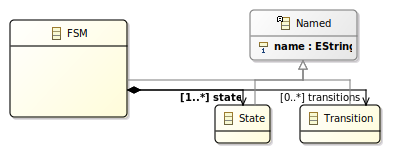
\includegraphics[width=\textwidth]{FSM0.pdf}
      \caption{Initial \metamodel.}
      \label{fig:FSM:Init}
    \end{subfigure}
    \hfill
    \begin{subfigure}[b]{0.45\textwidth}
			\centering
      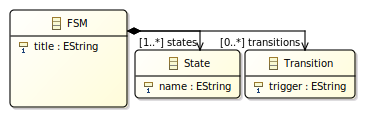
\includegraphics[width=\textwidth]{FSM1.pdf}
      \caption{\textbf{Step 1:} Specifying relevant \textsf{name}s}
      \label{fig:FSM:Relevant}
    \end{subfigure}
    \hfill
    \begin{subfigure}[b]{0.45\textwidth}
			\centering
      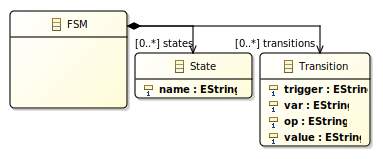
\includegraphics[width=\textwidth]{FSM2.pdf}
      \caption{\textbf{Step 2:} Adding rudimentary information for guards}
      \label{fig:FSM:Guard}
    \end{subfigure}
    \hfill 
		\begin{subfigure}[b]{0.45\textwidth}
			\centering
      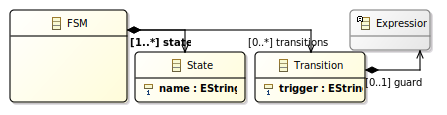
\includegraphics[width=\textwidth]{FSM3.pdf}
      \caption{\textbf{Step 3:} Specifying a fully-fledged \textsf{Expression} for \textsf{guard}s.}
      \label{fig:FSM:Expression}
    \end{subfigure}
    \caption{Three evolution steps for the \textsf{FSM} \metamodel}
    \label{fig:FSM}
\end{figure*}


\MA{Not finished yet! It needs:
\begin{itemize}
	\item Figures for views;
	\item Eventually, explanation that all is synced with the internal model.
	\item Explanation on the impact of the changes
\end{itemize}
Note that I completely failed at finding evolution steps that are purely ``atomic'':
any \emph{meaningful} (in the sense of my explanation here) evolution step, even
for such a small example, actually uses \textbf{a list of} atomic/composite 
changes!!! This was only partially discussed in our last meeting...}

This Section describes a small, yet representative example of \metamodel
evolution steps on a popular \textsc{Dsl}, the Finite State Machine (\textsf{FSM}).
Note that we simplify the \metamodels and corresponding \viewtypes, to focus 
the discussion only on the parts relevant to co-evolution. 

A methodologist starts with the simple version depicted in Figure \ref{fig:FSM:Init}:
an \textsf{FSM} consists of \textsf{State}s and \textsf{Transition}s. Each class
inherits a \textsf{name} that denotes the \textsf{FSM}'s title, the \textsf{State}'s
name, and the \textsf{Transition}'s trigger. From this initial version of \textsf{FSM},
the methodologist defines two views (types). The first one is \emph{visual},
and relies on different \textsf{Rountangle}s and \textsf{Arrow}s to depict the 
\textsf{FSM}, and provides two counters displaying the total number of \textsf{State}s
and \textsf{Transition}s in a model. The second one is \emph{textual}, and offers
a compact representation where \textsf{Transition}s are ``embedded'' inside 
\textsf{State}s. The specification, and an \textsf{FSM} model consisting of two
\textsf{State}s with three \textsf{Transition}s, are depicted in Figure \ref{fig:VT0}.

In a first evolution step, the methodologist refines the \textsf{FSM} metamodel,
after noticing that the inherited \textsf{name}s actually play different functions,
by  \emph{pushing down} the \textsf{name} attribute and \emph{renaming} it where
appropriate. This evolution step does not impact the \viewtypes, but rather the
way information in views is computed: for example, displaying the \textsf{TextArea}
above an \textsf{Arrow} in the visual representation needs to be updated from
\texttt{self.name} to \texttt{self.\textbf{trigger}}. 

In a second evolution step, the methodologist wants to extend \textsf{FSM}'s 
behaviour by adding a rudimentary representation for guards that may prevent
triggering a \textsf{Transition} when evaluated to \texttt{false}. For this purpose,
three new attributes are \emph{created} in \textsf{Transition}, allowing to capture
simple expressions over \textsf{var}iables, using boolean and numeric \textsf{value}s
(e.g. \textsf{v = 10} or \textsf{k or l}). After that, \textsf{FSM}'s views, as 
depicted in Fig. \ref{}, may still be valid wrt. the evolved \metamodel 
(assuming the lack of guard is interpreted as a trivial \textsf{true} guard),
but \viewtypes still need to reflect this new information by \emph{ADD}ing new 
entities. 

In a final evolution step, the methodologist, confident with the implemented
execution engine, specifies a fully-fledged \textsf{Expression} model,
allowing a \textsf{Transition} to possess a \textsf{guard}, thus \emph{deleting}
the extra attributes added in the previous step.


\begin{figure*}
    \centering
    \begin{subfigure}[b]{0.45\textwidth}
			\centering
      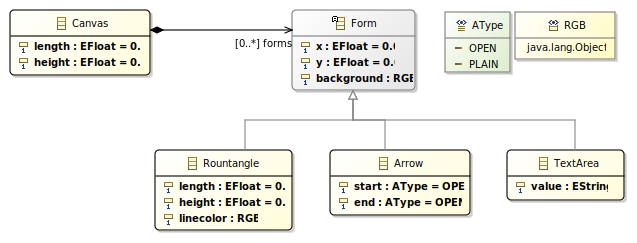
\includegraphics[width=\textwidth]{Visual.pdf}
      \caption{Viewtype for the \emph{visual} representation}
      \label{fig:FSM:Init}
    \end{subfigure}
    \hfill
    \begin{subfigure}[b]{0.45\textwidth}
			\centering
      \includegraphics[width=0.65\textwidth, page=1, clip, trim=0cm 11.6cm 21.4cm 0cm]{VT.pdf}
      \caption{A \textsf{Simple FSM} model conforming to the \emph{visual} \viewtype}
      \label{fig:FSM:Relevant}
    \end{subfigure}
    \hfill
    \begin{subfigure}[b]{0.45\textwidth}
			\centering
      \includegraphics[width=0.6\textwidth, page=2, clip, trim=0cm 14cm 26cm 0cm]{VT.pdf}
      \caption{Viewtype for the \emph{textual} representation \MA{Write the BNF spec!}}
      \label{fig:FSM:Guard}
    \end{subfigure}
    \hfill
    \begin{subfigure}[b]{0.45\textwidth}
			\centering
      \includegraphics[width=0.6\textwidth, page=2, clip, trim=0cm 13.5cm 26cm 0cm]{VT.pdf}
      \caption{A \textsf{Simple FSM} model conforming to the \emph{textual} \viewtype}
      \label{fig:FSM:Guard}
    \end{subfigure}
    \caption{Two \viewtypes, and associated views depicted the \textsf{Simple FSM} model.}
    \label{fig:FSM}
\end{figure*}

\section{Suggesting Changes In View(s Types)}
\label{sec:Suggestion}

Figure \ref{fig:Suggestion} depicts a \metamodel that capture the
required elements for helping methodologists improve their designs.
On the following, we assume that a methodologist is evolving a \metamodel
\textsf{MM} that is linked to a family of viewtypes $(\mathsf{VT}_i)$ 
(with $i\in [1..n]$). Note that in the discussion above, when we discuss
\textsf{MM}'s (meta-)elements, we consider \textsf{MM} as a \emph{model}
conforming to a particular meta-\metamodel (such as \textsc{Mof} \ref{}):
we therefore discuss changes on \textsf{MM}'s packages, classes (e.g. 
\textsf{FSM} or \textsf{State} in our example) and their structural features
(such as the attribute \textsf{name} or the reference \textsf{src}).

A \textsf{Suggestion} is the core element of our approach, and contains three 
parts: a \textsf{Change}, some \textsf{Relation}s, and a list of 
\textsf{Recommendation}s. 
%
As detailed in Figure \ref{fig:Change}, a \textsf{Change} captures the nature of
alterations operated on \textsf{MM}'s meta-elements. A \textsf{Change} refers 
to an \textsf{Operator} that may be parameterised with extra data, and contains 
contextual information (in \textsf{ApplicationPattern}). 
Change \textsf{Operator}s may target \emph{any} instanciable metamodel element, 
thus referring to the class \textsf{NamedElement} in \textsc{Mof}. Note that we 
will distinguish between \emph{primitive} and \emph{complex} \textsf{Operator}s,
depending on the number of such \metamodel elements an \textsf{Operator} acts on.

\textsf{Relation}s contain traceability links between \textsf{MM}'s and \viewtypes'
meta-elements. Note that these links may target \emph{several} meta-elements on 
the same \viewtype $\mathsf{VT_i}$, but also on \emph{various} \viewtypes. 

A \textsf{Recommendation} captures possible actions a methodologist may perform
to realign a \viewtype after a change. Note that a \textsf{Suggestion} may 
associate \emph{no} \textsf{Recommendation}s, in case a \textsf{Change} has no
impact on \viewtypes; or \emph{several} \textsf{Recommendation}s for the same 
\textsf{Change}, depending on the complexity of the \textsf{Change}, and how 
many \viewtypes are concerned by the \textsf{Change}.

The rest of this Section details each part in a \textsf{Suggestion}; a summary
is presented in Table \ref{tab:suggestions}.

\subsection{Change}
\label{sec:Suggestion:Change}

\begin{figure}[t]
    \centering
    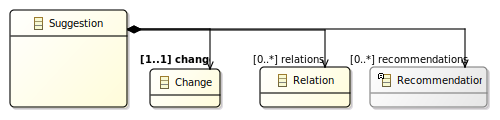
\includegraphics[width=\columnwidth]{images/Suggestion.pdf}
    \caption{A \textsf{Suggestion} holds for a single \textsf{Change} linked to 
		elements in a View Type through \textsf{Relation}s, and consists of a set of \textsf{Recommendation}s.}
    \label{fig:Suggestion}
\end{figure}

A \textsf{Change} refers to an \textsf{Operator} that may be parameterised with 
extra data, and contains contextual information (in \textsf{ApplicationPattern}\LC{what is meant by this? ApplicationPattern is not visible in any Figure, and Googling it, is not immediately clear which if any specific design pattern it refers to, if that's what's intended}). 
Change \textsf{Operator}s may target \emph{any} instantiable \metamodel element, 
thus referring to the class \textsf{NamedElement} in \textsc{Mof}. Note that we 
will distinguish between \emph{primitive} and \emph{complex} \textsf{Operator}s,
depending on the number of such \metamodel elements an \textsf{Operator} acts on.

Since \viewtypes are structurally \metamodels, we reviewed the literature to
identify relevant change \textsf{Operator}s. In our work, we integrate all 27 \textit{primitive} and seven of the 34 \textit{complex} operators in the change catalogue proposed by Herrmannsdoerfer et al.~\cite{herrmannsdoerfer_extensive_2011}.
These seven were selected because they constitute 72\% of all complex changes appearing in a large case study (cf. \cite{khelladi_detecting_2015}). 

\textsf{Operator}s are enriched with a \emph{severity}: \emph{Major}
(abbreviated as \textsf{M}), \emph{miNor} (\textsf{N}) and \emph{Ignore} 
(\textsf{I}). 
When applied to a \metamodel, the \textsf{Operator}s in \textsf{I} have no effect
on the corresponding \viewtypes; \textsf{Operator}s that can break the relationship
between \textsf{MM }and its \viewtypes are categorised as \textsf{M}; the rest of the
\textsf{Operator}s are \textsf{N}, since they are not breaking and can enrich 
the \viewtypes with additional information.\LC{Idea I've applied to table, to save space/cognitive load on table: dropped the 'I' operator rows from the table completely; instead adding next sentence here:} The seven \textsf{Operator}s \textsf{Make/Drop Class Abstract}, \textsf{Make/Drop Attribute Identifier}, \textsf{Make/Switch Reference Composite}, and \textsf{Pull Property} are of type \textsf{I} and hence not included in Table~\ref{tab:suggestions} of suggestions per change operator.

\begin{figure}[t]
    \centering
    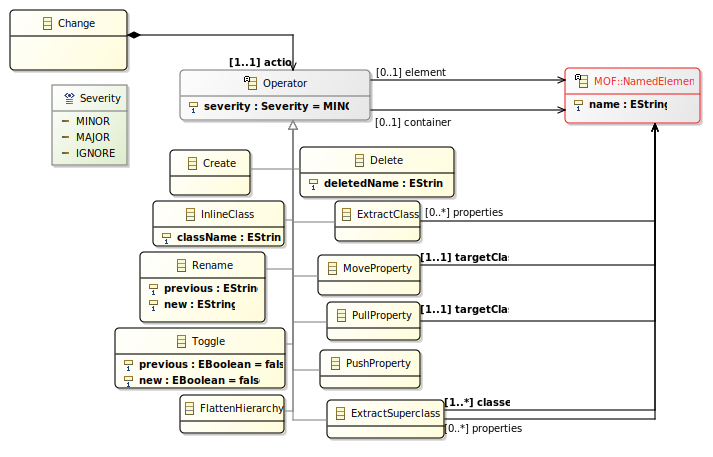
\includegraphics[width=\columnwidth]{Change.pdf}
    \caption{Possible \textsf{Operator}s for \metamodel evolution.}
    \label{fig:Change}
\end{figure}

The evolution steps of Figure \ref{fig:FSM} make use of different \textsf{Operator}s.
\begin{itemize}
	\item In Step 1 (depicted from Figure \ref{fig:FSM:Init} to \ref{fig:FSM:Relevant}),
	the following sequence of \textsf{Operator}s is applied:
	$$\langle \mathsf{PushProperty} \cdot \mathsf{Rename} \cdot \mathsf{Rename} \rangle$$
	First, \textsf{PushProperty} pushes down $\mathsf{Named} \squaredots \mathsf{name}$
	(i.e. pushes down the \textsf{element} \textsf{name} in the \textsf{container}
	\textsf{Named})
	into each subclass (namely, \textsf{FSM}, \textsf{State} and \textsf{Transition});
	then \textsf{Rename} is applied to the \textsf{element} \textsf{name}, 
	located respectively in \textsf{container}s $\mathsf{FSM}$ and 
	$\mathsf{Transition}$, thus obtaining the result of Figure \ref{fig:FSM:Relevant}.
	
	\item Step 2 only consists of the following \textsf{Operator} sequence:
	$$\langle \mathsf{Create} \cdot \mathsf{Create} \cdot \mathsf{Create} \rangle$$
	where each \textsf{Operator} adds a new Attribute \textsf{element} in 
	\textsf{container} \textsf{Transition}, ending up in the situation of
	Figure \ref{fig:FSM:Guard}.
	
	\item Step 3 requires a longer sequence of \textsf{Operator}s, since it creates
	a new class hieararchy under \textsf{Expression}. However, this sequence may
	start with the following:
	$$\langle \mathsf{Delete}^3 \cdot \mathsf{Create}^2 \cdot \ldots \rangle$$
	The initial \textsf{Delete}s undo the \textsf{Create} operations of Step 2
	(thus, referring to the same \textsf{element}s and \textsf{container}); and
	the two following \textsf{Create}s create the new \textsf{Expression} class
	(with the default package as a \textsf{container}) and the \textsf{guard}
	reference (with \textsf{Transition} as a \textsf{container}).
\end{itemize}
With these examples, we immediately notice that some \textsf{Operator}s
in a \textsf{Change} sequence may depend on previous ones (e.g. \textsf{Rename}
in Step 1 should only be performed after \textsf{PushProperty}); while others
may freely commute (e.g. the \textsf{Create} in Step 2 may be performed in any 
order).
\subsection{Relations}
\label{sec:Suggestion:Relation}


\subsection{Recommendation}
\label{sec:Suggestion:Recommendation}

Wheras an \textsf{Operator} concerns \textsf{MM}, a \textsf{Recommendation} 
describes an action a methodologist may perform on \textsf{VT} in order to
co-evolve \viewtypes. 
In our approach, we issue a \textsf{Recommendation} for each \viewtype element 
\textsf{impacted} by an \textsf{Operator}. We identified four kinds of \textsf{Action}s: 
\begin{itemize}
	\item a \textsf{DEL}ete action that a \viewtype element is no longer associated
	to an \textsf{MM} element, and thus may be deleted;
	\item an \textsf{ADD} action suggests to create a new element in the \viewtype
	to reflect a newly created \textsf{MM} element;
	\item an \textsf{UP}date action changes the (String) value of a \viewtype element;
	\item a \textsf{MOVE} action suggests to move a \viewtype element from a \textsf{src}
	(source) to \textsf{tgt} (target) container.
\end{itemize}
Note that each \textsf{Recommendation} action stores a \textsf{name} (which, for
\textsf{UP}date, corresponds to the new value, whereas \textsf{previous} 
indicates the original one), as well as its \textsf{container}, but also 
indicates the \textsf{type} of the \viewtype meta-element the 
\textsf{Recommendation} is performed on.

\autoref{tab:suggestions} provides the details of each \textsf{Recommendation} 
following the list of \textsf{Operator}s we identified in Sec. 
\ref{sec:Suggestion:Change} and commented in the next section.

\begin{figure}[t]
    \centering
    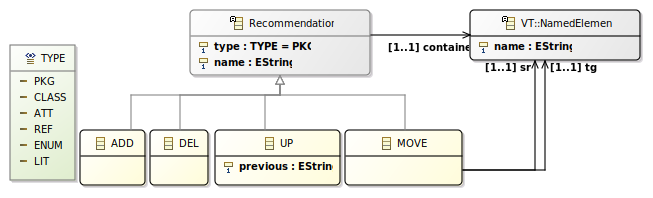
\includegraphics[width=\columnwidth]{Recommendation.pdf}
    \caption{\textsf{Recommendation}s actions suggested after a \textsf{Change}
    e.g. in Step 1, \textsf{ADD} Attribute \textsf{name} in \textsf{Transition} 
		\HM{i think it might be useful to include the word 'action' in the caption 
		as this figure is for that purpose. also do we have a sentence or so in the 
		running text explicitly mentioning about the difference between action and 
		operation?}
		\MA{Added ``action'' in caption. \textbf{What is an ``operation''}? Normally
		we only talk about \textsf{Operat\textbf{or}s!!!} If this is what you mean, yes: start of \S IV.C}}
    \label{fig:Recommendation}
\end{figure}


\section{Approach} 
\label{sec:Approach}

\LC{TODO: talk about domain-specific approach / refinements to approach, considering state charts }
\MA{The description of the MM for \textsf{Suggestion} has been lifted up on \S \ref{sec:Suggestion}. This Section should now
detail Table \ref{tab:suggestions}, and explain the \emph{choices} operated by our \textsf{Recommendation}s: \textbf{\emph{Why}}, 
when a MM element of this type is \emph{craeted}, do we suggest the \textsf{ADD}ition of ... in the \textsf{VT}? In other words,
this Section details the "content" of the \textsf{Suggestion} MM!}

As explained in Sec. \ref{sec:Suggestion:Change}, based on the how \viewtypes are affected we grouped the MM change \textsf{Operator}s into three severity categories: \textit{MAJOR}, \textit{MINOR} and \textit{IGNORE}. The following \textsf{Operator}s are categorised as \textsf{IGNORE}: \textit{Delete Package}, \textit{Make/Drop Class Abstract}, \textit{Make/Drop Attribute Identifier}, \textit{Make/Switch Reference Composite}, \textit{Make/Switch Reference Opposite} and \textit{Pull Property}. These operators are excluded from Table~\ref{tab:suggestions}, which lists the chosen MM change \textsf{Operator}s and corresponding \textsf{Recommendation}s, since they don't result into any \textsf{Recommendation}s.



% The following \textsf{Operator}s have severity \textsf{IGNORE}, and are 
% therefore not included in Table~\ref{tab:suggestions} since they do result
% in no \textsf{Recommendation}s: \textsf{Make/Drop Class Abstract}, 
% \textsf{Make/Drop Attribute Identifier}, \textsf{Make/Switch Reference Composite},
% and \textsf{Pull Property}.




Among the primitive operations the creation of various entities are of minor severity as they do not influence the existing relation between the \metamodel and corresponding \viewtypes. For the creation of package, class, data type, and enumeration, we only notify the modeller about the addition of these entities. 
According to the \metamodeling formalism proposed by \cite{herrmannsdoerfer_extensive_2011}, attributes and references, and literals, have composition relation with resp. classes and enumerations. Therefore, in the event of the creation of these entities, we first identify the \viewtypes that reference the corresponding container (i.e., class or enumeration) and suggest the addition of the new entities for these \viewtypes.

The deletion of a package is possible iff it is empty and therefore, this operation can be safely ignored. Deleting class, feature, data type, and enumeration can have major consequence if these entities are referred from one or more related \viewtypes as the partial representation relation with the corresponding \metamodel no longer holds. Therefore, the suggestion is to remove these entities also from the \viewtypes.

The \textit{Make Class Abstract} and \textit{Drop Class Abstract} are about making an existing class abstract and vice versa. As these operations only changes the abstraction without modifying the list of features, they can be ignored in the context of \viewtype co-evolution. 

The deletion of an opposite reference removes access to the referenced entity from the referencing one. The corresponding suggestion is to remove the references also from the \viewtype. \textit{Merge Literal} removes a literal and replaces its occurrence with another one. Therefore, applying this operations triggers the suggestion to replace the deleted literal with an existing one in the \viewtype. \textit{Rename} and \textit{Change Package} operators generate suggestions to do the same (i.e., renaming and changing package location) on the related \viewtypes.

The \textit{Add Super Type} and \textit{Remove Super Type} operators adds and removes inherited features from an existing class. Accordingly, the corresponding suggestion suggests the addition or removal of inherited features wherever the child class is referenced in the \viewtype. Although the suggestion for the former is of minor severity, the removal of features can break the \viewtype and hence, is classified as major.

The \textit{Make Attribute Identified} and \textit{Drop Attribute Identifier} operators adds or removes a constraint that ensures the uniqueness of the attribute values. The \textit{Make Reference Composite} and \textit{Drop Reference Composite} adds or removes the containment restriction for an reference. Since, these are instance level constraints, they do not influence the \viewtype and therefore, can be ignored.

\HM{Discuss \textit{Make ref opposite and drop ref opposite}} \MA{I have some arguments to say that we could ignore these in a first attempt, because "opposite"s may always be computed, assuming you have a "decent" meta-metamodel API (as EMF/Ecore provides, among others).}\LC{I agree.}

The \textit{Move Property} operator triggers the suggestion to update the corresponding location in the \viewtype. Pushing a property down in the hierarchy removes the property from the super class and therefore, it needs to be removed from the \viewtype wherever it is referred using a reference of the super class. The \textit{Pull Up} operator can be applied iff the corresponding feature is present in all the child classes. Since the feature is still accessible via inheritance, this does not trigger any suggestion for the related \viewtypes.

Extracting super class does not influence the effective set of features and therefore, triggers a minor suggestion for replacing some occurrences of the child class reference with the parent. The \textit{Flatten Hierarchy} moves all the features from the parent to the child classes and deletes the parent class. Therefore, this triggers a major suggestion for replacing all the references of the removed super class with the appropriate child class reference. Since the effective features of the child classes remain the same before and after fattening, we offer no suggestion for the child classes. The \textit{Extract Class} operator groups a set of features into a new delegate class and replaces their occurrences with a reference to the delegate class. The \textit{Inline Class} operator is the exact opposite of \textit{Extract Class}. Both triggers a major suggestion of adapting the location of any related feature referenced in the \viewtype.

\begin{table*}[ht!]
\caption{Suggestions per change operator. The Primitive and Complex operators are denoted respectively with P and C. \MA{Give a legend for the abbreviations in "Type" and "Severity" columns. Similarly, the "TYPE" values are never explained in the text (and should be part of the legend as well).}\HM{group all none suggestions}} \label{tab:suggestions}
\centering
\begin{tabular}{|l|c|p{.33\linewidth}|p{.31\linewidth}|c|}
\hline
Operator & Type & Condition to offer suggestion & Suggestion & Severity \\ \hline \hline

Create Package $(p)$&  
\multirow{8}{*}{P} & 
\multirow{8}{*}{\parbox{\linewidth}{The container of $x$ is referred in the \viewtype, where $x \in \{p, c, dt, e, r, or, a, l\}$}} &      
\multirow{8}{*}{Suggest $ADD(x)$ in the \viewtypes} &
\multirow{8}{*}{N} \\ \cline{1-1}
Create Class $(c)$&  &    &      &             \\ \cline{1-1}
Create Data Type $(dt)$&  &    &      &             \\ \cline{1-1}
Create Enum $(e)$&    &  &      &             \\ \cline{1-1}

Create Reference ($r$)& &  &      &             \\ \cline{1-1}
% \multirow{4}{*}{P} &    
% \multirow{4}{*}{\parbox{\linewidth}{Containers (i.e., package, class) to which the entity is added are referenced from the \viewtype}} &      
% \multirow{4}{*}{\parbox{\linewidth}{Suggest the addition of the new entities in the \viewtype}} &
% \multirow{4}{*}{N} \\ \cline{1-1}
Create Opposite Ref. ($or$)&   &   &      &             \\ \cline{1-1}
Create Attribute ($a$)&  &    &      &             \\ \cline{1-1}
Create Literal ($l$)&    &  &      &             \\ \hline

% Delete Package  & P &
% None & None. & N \\ \hline

Delete Class ($c$)& \multirow{4}{*}{P} & 
\multirow{4}{*}{\parbox{\linewidth}{$x$ is referenced in the \viewtype, where $x \in \{c, f, dt, e\}$}} &
\multirow{4}{*}{Suggest $DEL(x)$ from \viewtype} & \multirow{4}{*}{M}           \\ \cline{1-1}
Delete Feature ($f$) &     & &      &             \\ \cline{1-1}
Delete Data Type ($dt$) &    &  &      &             \\ \cline{1-1}
Delete Enum ($e$) &   &   &      &             \\ \hline

%Make Class Abstract  & \multirow{2}{*}{P} & \multirow{2}{*}{None}     & \multirow{2}{*}{None}     & \multirow{2}{*}{I} \\ \cline{1-1}
%Drop Class Abstract  &  & &  & \\ \hline

Delete Opposite Ref. ($or$) & P &  \Viewtype refers the referencing class & Suggest referenced class and corresponding features not accessible & M            \\ \hline
Merge Literal  ($l$)& P&  $l$ is referenced in \viewtype    & Suggest the $UP$dating $l$ with $l^\prime$, where $l$ and $l^\prime$ are contained in the same \textit{Enum} & M            \\ \hline
Rename  & P& Old name $s$ is referred in the \viewtype  &  Suggest $UP$dating $s$ with $s^\prime$ where $s^\prime$ is the current name & M \\ \hline
Change Package ($p$) & P& $x$ is referred in \viewtype, where $x\in\{p, t, dt, e, c\}$ and $x$ was contained in $p$ & Suggest $MOVE$ of $x$ from $p$ to $p^\prime$, where $p^\prime$ is the current package & M \\ \hline
Add Super Type ($t$) & P& $t_c$ is referred in \viewtype, where $t_c$ is a child type of $t$ & Suggest $ADD(f^*)$, where $f^*$ is the set of features contained in $t$ & N  \\ \hline
Remove Super Type ($t$) & P& $t_c$ is referred in \viewtype, where $t_c$ is a child type of $t$ & Suggest $DEL(f^*)$, where $f^*$ is the set of features contained in $t$ & M \\ \hline
%Make Attr. Identifier   & \multirow{4}{*}{P} &  \multirow{4}{*}{None}    &  \multirow{4}{*}{None}    & \multirow{4}{*}{I}            \\ \cline{1-1}
%Drop Attr. Identifier  & &      &      &     \\ \cline{1-1}
%Make Ref. Composite  & &      &      &             \\ \cline{1-1}
%Switch Ref. Composite  & &      &      &             \\ \hline
% Make Ref. Opposite  & P&  None\LC{Remove this and next line, see arguments Moussa in running text}    &   None   &             \\ \hline
% Drop Ref. Opposite  & P&   None   &    None  &             \\ \hline
Move feature ($f$) & C &  $f$ is referred in \viewtype  & Suggest $MOVE$ $f$ from $c_s$ to $c_d$, where $c_s$ and $c_d$ are previous and current container classes& M \\ \hline
Push feature ($f$)  & C & $f$ is referred in \viewtype using a reference of $c_s$, where $c_s$ is a super class from which $f$ was pushed to all its child classes $c_d$& Suggest $DEL(f)$ or $MOVE$ $f$ from $c_s$ to $c^\prime$, where $c^\prime\in c_d$   & M \\ \hline
%Pull Property   & C & None & None & I \\ \hline
Extract Super Class  & C & Child classes referred in \viewtype  & Suggest possible replacement of child classes with newly created super class & N  \\ \hline
Flatten Hierarchy   & C & Removed super class is referenced in \viewtype &   Suggest removal of super class and replace all of its occurrences with appropriate child class   &  M           \\ \hline
Extract Class   & C & Extracted features from the delegate class are referred in \viewtype & Suggest the moving of features to the delegate class from the original class & M \\ \hline
Inline Class   & C & Delegate class is referenced in \viewtype & Suggest moving of features from delegate class to class that referenced the delegate class & M            \\ \hline

\end{tabular}
\end{table*}
\section{Formalization}
\label{sec:Formalization}
In this chapter we define the terms suggestion and applicable suggestion. We introduce possible ways to refine a suggestion and to add domain specific knowledge.

\begin{definition}[Suggestion]
We define a suggestion $SUG$ as a 4-Tuple of a type of a change on the \metamodel $MMC$, a view generation transformation $VGT$, constraints $CON$ and a suggestion content $SUC$. Short: $SUG = (MMC, VGT, CON, SUC)$
\end{definition}
Possible $MMC$ are defined in \cref{tab:suggestions}. A suggestion always contains one change. Change sequences that have domain semantics should define a new complex change, because the contained domain knowledge is interesting for other analyses besides suggestions. The view generation operators $VGO$ are defined in \cref{fig:model-query-operators}. They can be combined to a $VGT$. $VGTs$ may form a hierarchy that can be used for the refinement of suggestions. The constraints are defined on either the \metamodel, its instance, the view generation operators or the target \metamodel. Constraints may also form a hierarchy for the refinement of suggestions. The $SUC$ is either a textual description of the suggestion or a change on the viewtype or a combination of both. Both is preferable as it enables the methodologist to precisely define the change on the \viewtype \metamodel as well as giving some rationale.

An example for a suggestion is \textit{(Create Attribute in metamodel, Select,  "viewtype is identity mapping of metamodel", ("As the viewtype is an identity mapping of the underlying metamodel, we suggest to update the viewtype to also include the new attribute.", Create Attribute in viewtype metamodel))}. A possible refinement could also include the $CON$ \textit{attribute is marked as hidden} which may semantically take precedence over the identity mapping and the suggestion contains the $SUC$ \textit{"As the attribute is marked as hidden, we suggest to not update the viewtype."}. Both $VGT$ and $CON$ enable the methodologist to include semantic domain specific knowledge into the suggestions.

\begin{definition}[Applicable Suggestion]
We define an applicable suggestion as a 3-Tuple of a suggestion, a transformation of the $VGT$($TVGT$) and a transformation between the $MMC$ and the $SUC$($TSUC$). Short $ASU = (SUG, TVGT, TSUC)$
\end{definition}
Note that the $SUC$ of an $ASU$ has to contain the definition of the change on the \viewtype \metamodel. The $TVGT$ transforms the $VGO$, e.g. by adding a newly created attribute as input. The $TSUC$ transforms the change on the \metamodel in a change on the \viewtype \metamodel. In the example above, the change on the \metamodel will be transformed by changing its target from the \metamodel to the \viewtype \metamodel. A suggestion can have multiple applicable suggestions from which the methodologist can chose the most appropriate one.
\input{chapters/Evaluation}
\section{Related Work}
\label{sec:RW}

\begin{itemize}
    \item \metamodel version co-existence (Alexander Egyed)
    \item MM to MM co-evolution
    \item database view co-evolution
\end{itemize}

\section{Conclusion} \label{sec:Conclusion}

In the context of view-based development, co-evolving \viewtypes together with corresponding \metamodels is crucial for maintaining the soundness and relevancy of the \viewtypes. This is especially important in industrial settings where in-house domain-specific languages evolve rather frequently. In this work, we 
% identified \LK{what does ``identify'' mean here, since we did not come up with them?} and \HM{i meant identified from the literature. but removed it to avoid confusion}
analyzed 34 \metamodel evolution operators---27 primitive and 7 complex ones---and proposed an approach for suggesting possible co-evolution actions on related \viewtypes for each \metamodel evolution operator. We first defined a conceptual model that associated a \metamodel change \textsf{Operator} with a set of \viewtype change \textsf{Recommendation}s, a \textsf{Relation} between the two, and a set of \textsf{Conditions}
% , which can be domain specific\LC{true for current paper?}\HM{not really, removed}, 
ensuring the validity of the recommendation (cf. \cref{sec:Suggestion}). Based on this conceptualization, we presented \viewtype co-evolution \textsf{Suggestion}s for each relevant \metamodel change \textsf{Operator} (cf. \cref{sec:Approach}). Furthermore, we understand that co-evolving \viewtypes and \metamodels require the co-evolution of the corresponding views and models. Therefore, we present and discuss several existing work that focuses on \metamodel/model and related co-evolution scenarios. 

We used the example of the Finite State Machine while presenting our approach for \viewtype/\metamodel co-evolution. Although, this example is adequate for explaining the approach, but it is too simplistic to be a viable method for evaluating its effectiveness.
% this example is sufficient for explaining the approach, it is too simple to serve as a viable means of evaluating the approach. 
Therefore, we aim to extend this work by evaluating the presented approach using one or more \metamodels applied in real-word situations such as the one from \textcite{braun_classification_2014}. Furthermore, we do not tackle the co-evolution of view generation transformations (VGT), which instantiates views based on a \viewtype, with the evolution of corresponding \viewtypes and \metamodels. This can partly be attributed to the present incompleteness of the VGT semantics. However, it remains an open research direction. 

\LC{TODO: Loek got to here.}

\LC{TODO: probably future work: talk about (i) more complex patterns to give better suggestions;
(ii) domain-specific approach / refinements to approach, with illustration on
state charts?}
\TW{I added an example in \cref{sec:Conditions}}

% discuss work, limitations, where it should go

% \st{viewtype transformations}


% Future work - make suggestions applicable 

\begin{comment}
\TW{TODO: remove the formalisation, cut the definition short and try to define the idea more precisely} \begin{definition}[Applicable Suggestion]
We define an applicable suggestion as a 3-Tuple of a suggestion, a transformation of the $VGT$($TVGT$) and a transformation between the $MMC$ and the $SUC$($TSUC$). Short $ASU = (SUG, TVGT, TSUC)$
\end{definition}
\HM{This definition seems unclear to me. I am also not sure of its relevance in the context of this work.} \TW{As discussed in the meeting, this definition is not part of the scope of this paper but future work on how to use our definitions. We may keep it as limitation or move its content to the future work section (a formal definition won't make sense there, but i think we should keep the ideas and present them.)}
Note that the $SUC$ of an $ASU$ has to contain the definition of the change on the \viewtype \metamodel. The $TVGT$ transforms the $VGO$, e.g. by adding a newly created attribute as input. The $TSUC$ transforms the change on the \metamodel in a change on the \viewtype \metamodel. In the example above, the change on the \metamodel will be transformed by changing its target from the \metamodel to the \viewtype \metamodel. A suggestion can have multiple applicable suggestions from which the methodologist can chose the most appropriate one.
\end{comment}


% \bibliographystyle{IEEEtran}
\printbibliography
\end{document}
